%%This is a very basic article template.
%%There is just one section and two subsections.
\documentclass{article}

\usepackage{lmodern}
\usepackage{xspace}

\usepackage{tikz}
\usetikzlibrary{fit}
\usetikzlibrary{backgrounds}
\usetikzlibrary{trees}
\usepackage{siunitx}

\usepackage{hyperref}

\newcommand{\email}[1]{\href{mailto:#1}{\nolinkurl{#1}}}

\title{
  {\normalsize \textsc{Design Document}\\[0.5em]}
  DarkVR: The Virtual Blind Reality
}

\author{Tom Brosch (17362104)}
\date{\email{brosch.tom@gmail.com}}

\newcommand{\darkvr}{\textsc{DarkVR}\xspace}

\begin{document}

\maketitle
%http://wiibrew.org/wiki/Wiimote/Library

\section{Introduction}

The project aims to create a virtual reality environment without visual cues and
without substituting visual cues by auditory cues (e.g. playing the sound of a
creaking door when you stand right in front of a door). The aim of the project
is, therefore, to create and experience a virtual world as close as possible to
how a blind would experience the real world.

This work is most closely related to the \textsc{Dialogue in the Dark}
project\cite{dialog}. \textsc{Dialogue in the Dark} is an exhibition which lets
non-blind people experience the world of the blinds and, thereby, raises
awareness for the problems blind people are faced everyday while navigate
through the world. Since the created environments are replicas build in an
indoor space, the number of scenarios that are rebuild is very limited. A
virtual reality can help bringing the blindness-experience to scenarios that are
too expensive to rebuild (e.g. navigating through an entire city) or too
dangerous (e.g. due to traffic).

The work is also related to video games for blinds. Video games for blinds can
be roughly classified into two categories: (1) games, which were initially
designed for blinds, and (2) games which have been made accessible to blinds.
Games of the first category often either use a combination of a
narrator, which introduces and describes a new scene, and auditory feedback,
which helps the user to navigate through the virtual environment (e.g. ``Der Tag
wird zur Nacht''\cite{dertag}); or use sound as the primary gaming concept (e.g.
``AudiOdyssey''\cite{audiodyssey}).

There has also been a great amount of research in how to make games accessible
for disabled people (e.g. \cite{chile, terraformers, secondlife,
tankcommander}). See \cite{survey} for a survey of accessible games. A common
method is to replace visuals with audio. This can be done on different levels of
abstraction. Audio cues are the least abstract way of replacing visuals with
audio. Audio cues are sounds that an object would make in the real world (e.g.
footsteps of a walking person). Auditory Icons or ear cons are sounds which are
associated with an object, even though the object would not make this sound in
the current situation (e.g. playing the sound of a creaking door when you stand
in front of it, even if the door is not moving). Sonification is used to
translate physical properties of an object into sound. These sounds are usually
artificial. Properties like pitch or frequency are used to represent other
properties like distance.

In contrast to the many attempts to making a virtual world accessible for the
blinds, this project aims to create an experience which is as closed as
possible to the real experience of blindness. Therefore, accessibility methods
like auditory icons/ear cons and sonifications are not used on purpose. Instead,
the user navigates through the world relying on 3D binaural audio and devices
like a virtual long cane or a virtual GPS localizer. \darkvr, therefore,
does not only give the possibility to experience blindness, it also gives the
possibility to try out imaginary devices that might help blinds in the
future to navigate and orientate in the real world.

\section{Design}

\subsection{Architecture Overview}

An overview of the program architecture is given in
figure~\ref{fig:architecture}. The core data structure for storing geometric and
auditory information about the scene is a scene graph. The project will use the
scene graph implementation of the \textsc{OpenSceneGraph} (OSG)
project\cite{osg}. The scene graph contains information about the terrain,
objects the user can interact with, a basic body model of the user, and the
geometric model of various devices, which the user uses to orientate in the
virtual environment. The remaining program modules can be divided into rendering
modules (e.g. for sound and graphics rendering), helper modules (e.g. the
collision detection module) and controllers. The first two classes form the
basic level, since they interact with the scene graph only. The controllers use
helper modules (e.g. the collision detection module). They process the user
input in order to make changes to the scene graph.

\tikzstyle{every node}+=[font=\sffamily]

%\usepackage{graphics} is needed for \includegraphics
\begin{figure}[htp]
\centering
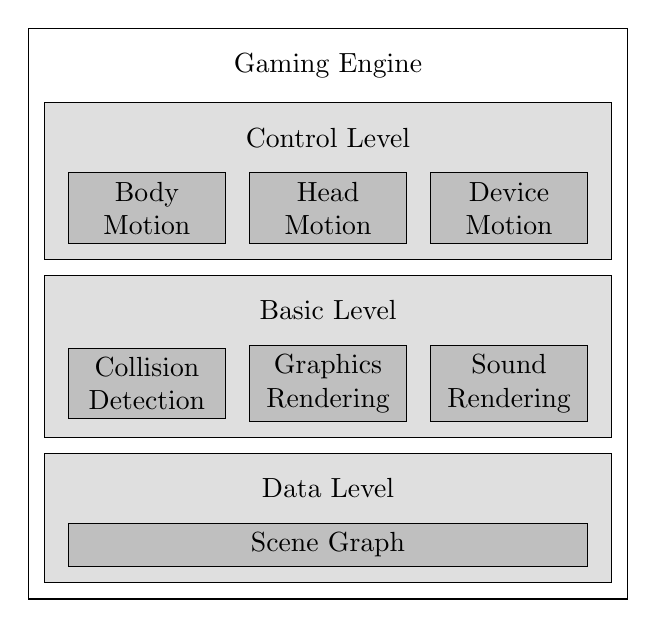
\begin{tikzpicture}

\tikzstyle{box}=[draw=black, align=center, minimum width=2cm, fill=lightgray]
\tikzstyle{fullbox}=[box, minimum width=6.6cm]
\tikzstyle{layer}=[draw=black, minimum width=7.2cm,inner
sep=0.2cm,fill=lightgray!50]
\tikzstyle{engine}=[draw=black, inner sep=0.2cm]

\matrix[column sep={2.3cm,between origins}] {
    & \node (engine) {Gaming Engine}; & \\[0.4cm]
    & \node (controllayer) {Control Level}; & \\[0.2cm]
    \node [box] (body) {Body\\Motion}; &
    \node [box] (head) {Head\\Motion}; &
    \node [box] (device) {Device\\Motion}; \\[0.6cm]
    & \node (basiclayer) {Basic Level}; & \\[0.2cm]
	\node[box] (collision) {Collision\\Detection}; & 
	\node[box] (graphics) {Graphics\\Rendering}; &
	\node[box] (rendering) {Sound\\Rendering}; \\[0.6cm]
	& \node (datalayer) {Data Level}; & \\[0.2cm]
	& \node[fullbox] (scenegraph) {Scene Graph}; & \\
};
\begin{scope}[on background layer]
	\node[layer, fit=(basiclayer)(collision)(graphics)(rendering)] {};
	\node[layer, fit=(controllayer)(body)(head)(device)] {};
	\node[layer, fit=(datalayer)(scenegraph)] (databox){};
	\node[engine, fit=(engine)(databox)] {};
\end{scope}
\end{tikzpicture}
\caption{Program architecture. The program is structured in a 3 level hierarchy.
Lower levels are independent of higher levels.}
\label{fig:architecture}
\end{figure}

An overview of the main control flow is given in figure~\ref{fig:mainloop}. The
core program runs in a main loop. The main loop calls the different controllers
which themselves poll inputs from the input devices and make changes to the
scene graph. At the end, the sound rendering module is called and the main loop
starts again.

\begin{figure}
\centering
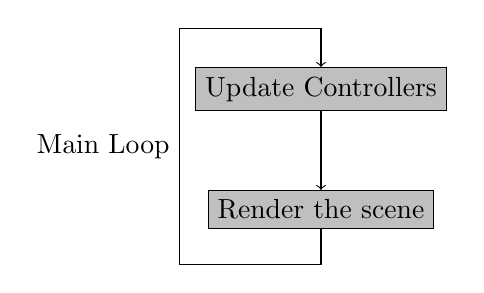
\begin{tikzpicture}

\tikzstyle{box}=[draw=black, align=center, fill=lightgray]

\matrix[row sep={1cm}] {
	\node[box] (update) {Update Controllers}; \\
	\node[box] (render) {Render the scene}; \\
};
\draw[->] (update)--(render);
\draw[black,->] (render) -- ++(0, -0.7cm) -- ++(-1.8cm, 0cm) --node[left] {Main
Loop} ++(0, 3cm) -- ++(1.8cm, 0cm) -- (update);
\end{tikzpicture}
\caption{The main program flow. First, all controllers are requested to update
their states. Then, the scene is rendered by calling all registered rendering
modules. These are the sound renderer and the optional graphics renderer.}
\label{fig:mainloop}
\end{figure}

\subsection{Data Layer: The Scene Graph}

The basic structure of the scene graph is shown in figure~\ref{fig:graph}.
There is a dedicated node for the head. This allows for head motion independent
of the whole body motion. The audio listener is attached to the head. Sound
sources can be added to the graph in order to add sounds to the scene. This is
done either static (e.g. for the terrain), or dynamic (e.g. in case of
triggered sounds due to collision).

\begin{figure}
\centering
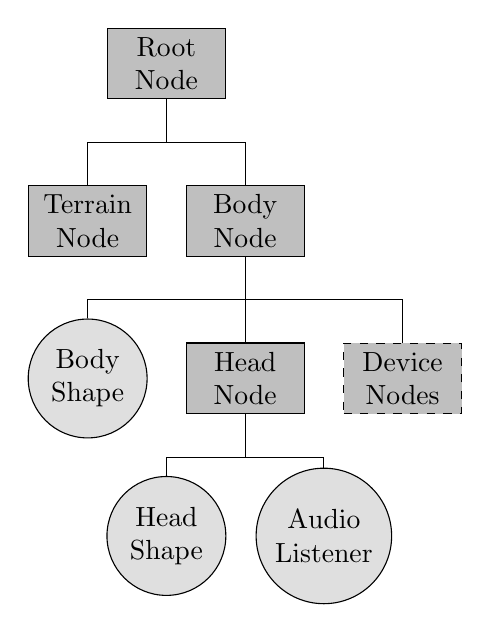
\begin{tikzpicture}[level distance=2cm, sibling distance=2cm]
%[grow via three points={
%one child at (0,-2) and two children at (-1,-3) and (1,-3)}, level distance=-1]

\tikzstyle{osgnode}=[align=center,draw=black, minimum
width=1.5cm,fill=lightgray]
\tikzstyle{osgelement}=[align=center,shape=circle,draw=black,fill=lightgray!50]

\node[osgnode] {Root\\Node}
[edge from parent fork down]
child {node[osgnode] {Terrain\\Node}}
child {node[osgnode] {Body\\Node}
	child {node[osgelement] {Body\\Shape}}
	child {node[osgnode] {Head\\Node}
		child {node[osgelement] {Head\\Shape}}
		child {node[osgelement] {Audio\\Listener}}
	}
	child {node[osgnode,dashed] {Device\\Nodes}}
};
\end{tikzpicture}

\caption{Basic structure of the scene graph. There is a dedicated node for the
head. This allows for head motion independent of the whole body motion. The
audio listener is attached to the head.}
\label{fig:graph}
\end{figure}

\subsection{Basic Layer}

Modules from the basic layer depend on the scene graph only. They provide basic
functionality which will be used by modules of higher layers.

\subsubsection{Collision Detection}

Collisions are calculated using the \textsc{Bullet Physics
Library}\cite{bullet}. Thereby, \textsc{osgBullet}\cite{osgBullet} acts as a
layer between \textsc{Bullet} and OSG and maps geometric
information from OSG to the internal geometric representation of
\textsc{Bullet}. The collision module is mainly used to detect the collision of
the moving user and his devices with the world.

\subsubsection{Graphics Rendering}

Graphics can be rendered for debugging and testing purpose. OSG is used to
render graphics, which uses \textsc{OpenGL}\cite{opengl} internally.

\subsubsection{Sound Rendering}

3D sound is rendered using the \textsc{FMOD Ex Programmer's API}
(FMOD)\cite{fmod}.
FMOD provides functions for placing sounds in a 3D environment and renders these
sounds according to the listeners position. It uses Head-Related Transfer
Function (HRTF) to simulate the filtering caused by the outer ear. FMOD features
a geometric engine to simulate sound occlusion and obstruction. I will use
\textsc{osgAudio}\cite{osgAudio} to map the OSG to the geometric model of FMOD.
The sound rendering engine also removes out-dated sound nodes from the scene
graph.

\subsection{Control Layer}

Modules from the control layer interact with the scene graph. They use modules
from the basic layer to perform certain tasks.

\subsubsection{Body Motion Controller}

The body motion controller reads inputs from the mouse and keyboard and
translates these events to body movement. The left and right arrow keys are used
to rotate the person \ang{30} to the left and the the right, respectively.
The up and down keys are used to move the person forwards and backwards,
respectively. It uses the collision detection module to detect collisions with
the environment. The movement controller moves the body node in the scene graph.
It also adds sound nodes to the scene graph if the person hits an object in the
world.

\subsubsection{Head Motion Controller}

The head movement controller reads input from the magnetic head tracker. It
moves the head node relative to the body node, without collision detection. The
audio listener is attached to the head. Thus, the position of sound sources
relative to the body remains constant even when the user moves the head
including head phones.

\subsubsection{Device Motion Controllers}

\paragraph{Long Cane} The long cane is simulated using the Wii Remote Controller
(Wiimote). The \textsc{wiiuse}
library\footnote{\url{http://sourceforge.net/projects/wiiuse/}} will be used to
get the 3D position of the Wiimote. The node of the virtual long cane will be
moved to reflection the current position of the Wiimote. The controller checks
for collisions of the cane with the world. If a collision is detected, a sound
node is added to the scene graph. Furthermore, the rumble feature of the Wiimote
will be used to give simple haptic feedback.

\newpage

\section{User Study}

\subsection{Research Questions}

The research questions can be divided into different categories. The first one
are technical questions.

\subsubsection{3D Audio}

\begin{enumerate}
  \item How convincing is the audio experience? (on a scale between 1 and 5)
  \item Which control setup works better: WASD + mouse or rather discrete
  movement using the arrow keys? (categorical)
  \item How precise can audio sources be spotted using 3D audio? (Here are
  different test scenarios possible: (1) relate different sources according to
  closer vs. farther to the user, more left vs. more right, higher vs. lower;
  (2) simple guessing game where the distance to an object has to be guessed
  when other sounds are given as reference points.)
\end{enumerate}

\subsubsection{Devices}

Subjective rating of different devices with regard to \ldots
\begin{enumerate}
  \item \ldots ease of use. Is the handling to complicated?
  \item \ldots usefulness. How good can you navigate using this device?
\end{enumerate}

Objective measurement of the performance in a way-finding game using different
devices. Measurable quantities are
\begin{enumerate}
  \item Time to complete the course.
  \item Number of body collision with objects that have to be avoided (e.g.
  other people, stepping into flowers, \ldots)
\end{enumerate} 

\subsection{Questionnaire}

\emph{Incomplete. Will be completed soon.}

\subsection{Ethics certificate}

\emph{Incomplete. Will be completed soon.}

\bibliographystyle{plain}
\bibliography{design}


\end{document}
